\section{Gnu Plot (\texttt{gnuplot})}

\texttt{gnuplot} is a utility that can be run on a variety of platforms (Linux,
macOS, Windows, and many more) used to generate high-quality plots and graphs.
Unlike Excel, \texttt{gnuplot} is used through the command-line --- the shell.
Although you can use it interactively, issuing commands and having the current
plot be redrawn, \texttt{gnuplot} is capable of running commands in batch,
lending itself very naturally for use in a \Bash{} script. To install
\texttt{gnuplot} on Linux:

\begin{shlisting}{}
$ sudo apt install gnuplot
\end{shlisting}

\texttt{gnuplot} is mostly used to plot data points in a file. The basic format
is very simplistic: just a series of $(x, y)$ coordinates on each line, separated
by whitespace.

\begin{pylisting}{Example data file: \texttt{example.dat}.}
1 5
2 4
3 3
4 2
5 1
\end{pylisting}

After you've created this file, start up \texttt{gnuplot}. This should open up
an interactive prompt. From here, all we need to do is specify what data file to
plot and how to plot it.

\begin{shlisting}{}
$ gnuplot

        G N U P L O T
        Version 5.4 patchlevel 2    last modified 2021-06-01

        Copyright (C) 1986-1993, 1998, 2004, 2007-2021
        Thomas Williams, Colin Kelley and many others

        gnuplot home:     http://www.gnuplot.info
        faq, bugs, etc:   type "help FAQ"
        immediate help:   type "help"  (plot window: hit 'h')

Terminal type is now 'qt'
gnuplot> plot "example.dat" with linespoints
\end{shlisting}

Entering this command into \texttt{gnuplot} should result in the plot popping up
in a window. We would also like to be able to export a plot to a file, say a
PDF. We'd also prefer if we didn't have to interactively type out what to plot
each time. There is where the non-interactive mode for \texttt{gnuplot} comes
in. We can create a file listing the commands we'd ordinarily issue to
\texttt{gnuplot} interactively and instruct it to output the plot to a PDF of
our choosing.

\begin{pylisting}{Example \texttt{gnuplot} file: \texttt{example.plot}.}
set terminal pdf
set output "example.pdf"
set xlabel "x"
set ylabel "y"
plot "example.dat" with linespoints
\end{pylisting}

We now redirect the contents of \texttt{example.plot} into \texttt{gnuplot},
which should generate the plot in a file named \texttt{example.pdf}. The plot
should resemble Figure \ref{figure:example}. We'll learn more about file
redirection when we discuss basic \Bash{} scripting in \S\ref{section:bash}.

\begin{shlisting}{}
$ gnuplot < example.plot
\end{shlisting}

\begin{figure}[bth]
  \centering
  % GNUPLOT: LaTeX picture with Postscript
\begingroup
  \makeatletter
  \providecommand\color[2][]{%
    \GenericError{(gnuplot) \space\space\space\@spaces}{%
      Package color not loaded in conjunction with
      terminal option `colourtext'%
    }{See the gnuplot documentation for explanation.%
    }{Either use 'blacktext' in gnuplot or load the package
      color.sty in LaTeX.}%
    \renewcommand\color[2][]{}%
  }%
  \providecommand\includegraphics[2][]{%
    \GenericError{(gnuplot) \space\space\space\@spaces}{%
      Package graphicx or graphics not loaded%
    }{See the gnuplot documentation for explanation.%
    }{The gnuplot epslatex terminal needs graphicx.sty or graphics.sty.}%
    \renewcommand\includegraphics[2][]{}%
  }%
  \providecommand\rotatebox[2]{#2}%
  \@ifundefined{ifGPcolor}{%
    \newif\ifGPcolor
    \GPcolorfalse
  }{}%
  \@ifundefined{ifGPblacktext}{%
    \newif\ifGPblacktext
    \GPblacktexttrue
  }{}%
  % define a \g@addto@macro without @ in the name:
  \let\gplgaddtomacro\g@addto@macro
  % define empty templates for all commands taking text:
  \gdef\gplbacktext{}%
  \gdef\gplfronttext{}%
  \makeatother
  \ifGPblacktext
    % no textcolor at all
    \def\colorrgb#1{}%
    \def\colorgray#1{}%
  \else
    % gray or color?
    \ifGPcolor
      \def\colorrgb#1{\color[rgb]{#1}}%
      \def\colorgray#1{\color[gray]{#1}}%
      \expandafter\def\csname LTw\endcsname{\color{white}}%
      \expandafter\def\csname LTb\endcsname{\color{black}}%
      \expandafter\def\csname LTa\endcsname{\color{black}}%
      \expandafter\def\csname LT0\endcsname{\color[rgb]{1,0,0}}%
      \expandafter\def\csname LT1\endcsname{\color[rgb]{0,1,0}}%
      \expandafter\def\csname LT2\endcsname{\color[rgb]{0,0,1}}%
      \expandafter\def\csname LT3\endcsname{\color[rgb]{1,0,1}}%
      \expandafter\def\csname LT4\endcsname{\color[rgb]{0,1,1}}%
      \expandafter\def\csname LT5\endcsname{\color[rgb]{1,1,0}}%
      \expandafter\def\csname LT6\endcsname{\color[rgb]{0,0,0}}%
      \expandafter\def\csname LT7\endcsname{\color[rgb]{1,0.3,0}}%
      \expandafter\def\csname LT8\endcsname{\color[rgb]{0.5,0.5,0.5}}%
    \else
      % gray
      \def\colorrgb#1{\color{black}}%
      \def\colorgray#1{\color[gray]{#1}}%
      \expandafter\def\csname LTw\endcsname{\color{white}}%
      \expandafter\def\csname LTb\endcsname{\color{black}}%
      \expandafter\def\csname LTa\endcsname{\color{black}}%
      \expandafter\def\csname LT0\endcsname{\color{black}}%
      \expandafter\def\csname LT1\endcsname{\color{black}}%
      \expandafter\def\csname LT2\endcsname{\color{black}}%
      \expandafter\def\csname LT3\endcsname{\color{black}}%
      \expandafter\def\csname LT4\endcsname{\color{black}}%
      \expandafter\def\csname LT5\endcsname{\color{black}}%
      \expandafter\def\csname LT6\endcsname{\color{black}}%
      \expandafter\def\csname LT7\endcsname{\color{black}}%
      \expandafter\def\csname LT8\endcsname{\color{black}}%
    \fi
  \fi
    \setlength{\unitlength}{0.0500bp}%
    \ifx\gptboxheight\undefined%
      \newlength{\gptboxheight}%
      \newlength{\gptboxwidth}%
      \newsavebox{\gptboxtext}%
    \fi%
    \setlength{\fboxrule}{0.5pt}%
    \setlength{\fboxsep}{1pt}%
    \definecolor{tbcol}{rgb}{1,1,1}%
\begin{picture}(7200.00,5040.00)%
    \gplgaddtomacro\gplbacktext{%
      \csname LTb\endcsname%%
      \put(814,704){\makebox(0,0)[r]{\strut{}$1$}}%
      \put(814,1218){\makebox(0,0)[r]{\strut{}$1.5$}}%
      \put(814,1733){\makebox(0,0)[r]{\strut{}$2$}}%
      \put(814,2247){\makebox(0,0)[r]{\strut{}$2.5$}}%
      \put(814,2762){\makebox(0,0)[r]{\strut{}$3$}}%
      \put(814,3276){\makebox(0,0)[r]{\strut{}$3.5$}}%
      \put(814,3790){\makebox(0,0)[r]{\strut{}$4$}}%
      \put(814,4305){\makebox(0,0)[r]{\strut{}$4.5$}}%
      \put(814,4819){\makebox(0,0)[r]{\strut{}$5$}}%
      \put(946,484){\makebox(0,0){\strut{}$1$}}%
      \put(1678,484){\makebox(0,0){\strut{}$1.5$}}%
      \put(2410,484){\makebox(0,0){\strut{}$2$}}%
      \put(3142,484){\makebox(0,0){\strut{}$2.5$}}%
      \put(3875,484){\makebox(0,0){\strut{}$3$}}%
      \put(4607,484){\makebox(0,0){\strut{}$3.5$}}%
      \put(5339,484){\makebox(0,0){\strut{}$4$}}%
      \put(6071,484){\makebox(0,0){\strut{}$4.5$}}%
      \put(6803,484){\makebox(0,0){\strut{}$5$}}%
    }%
    \gplgaddtomacro\gplfronttext{%
      \csname LTb\endcsname%%
      \put(209,2761){\rotatebox{-270}{\makebox(0,0){\strut{}y}}}%
      \put(3874,154){\makebox(0,0){\strut{}x}}%
      \csname LTb\endcsname%%
      \put(5816,4646){\makebox(0,0)[r]{\strut{}"example.dat"}}%
    }%
    \gplbacktext
    \put(0,0){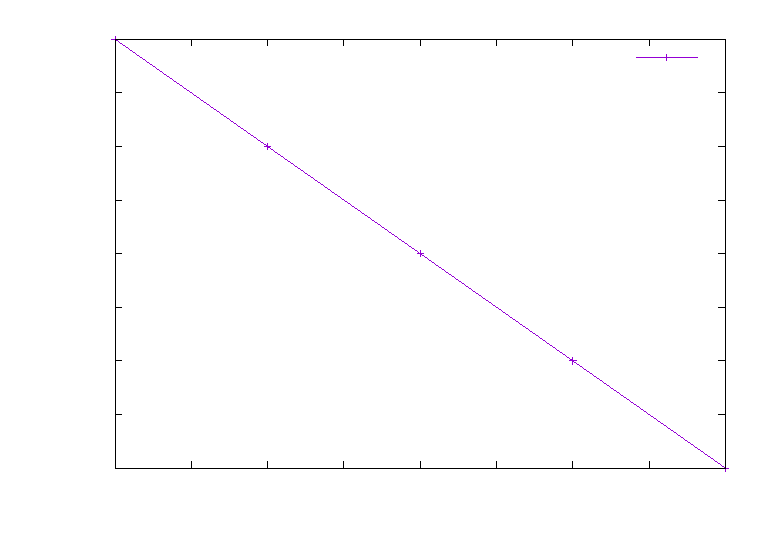
\includegraphics[width={360.00bp},height={252.00bp}]{figures/example}}%
    \gplfronttext
  \end{picture}%
\endgroup

  \caption{\label{figure:example}
    Example plot generated by \texttt{gnuplot}.
  }
\end{figure}

You can learn more about \texttt{gnuplot} and view more extensive examples,
respectively, with the following links:

\centerline{\url{http://gnuplot.info/documentation.html}}
\centerline{\url{http://gnuplot.info/demos/}}

There is also a built-in help system in \texttt{gnuplot}. Just type
``help'' when you are in interactive mode.

Do you have to use \texttt{gnuplot} for your course assignments? Yes. What about
Excel? No. What about some random online tool? No. You have to learn and use a
\Unix{} command line tool. If you are extremely insistent on not using
\texttt{gnuplot}, you can use \texttt{matplotlib} for Python as an alternative.
But you're on your own there.
